Working on financial problems is interesting on many levels. There is a large number of markets and it is easy to get the corresponding data even from years back.\footnote{%
	Although there are differences in the quality of the data resulting in a gap between freely available and commercial sources.}
What is measured is mostly \emph{value} and even though this is only an abstract concept its quantified by currencies which again opens the possibility of comparison between markets, assets etc.
There is also a large number of mathematical models and techniques often with intriguing results.

But even though all this formalization conveys a sense of order, one must not forget that markets are something created by humans. Therefore financial research is also related to the social sciences and besides all assumed efficiencies is subject to human emotion. As a result financial markets are ever-changing and nonlinear in their behavior.

Machine learning is about algorithms to enable computers to learn from existing data, allowing them e.g. to make predictions. In theory this could partly relieve human experts from adapting to market changes. For modeling financial data especially one technique might be useful: artificial neural networks with multiple layers -- recently rebranded as \emph{deep learning} -- already showed promising results in other works (e.g. \cite{Niaki-2013}).

First some necessary background for finance as well as deep learning is given. Using this knowledge, a description of the problem itself follows. Next comes the experimental part, evaluating data structure and model selection. Finally the results and findings are summarized, concluding this work.

On a technical note, the underlying code was written in Python~3 using Google's TensorFlow machine learning library.\cite{tensorflow2015-whitepaper} \\
The code is available at: \url{https://github.com/leyhline/vix-term-structure}

\section{Financial background}
\label{sec:financial-background}

The financial sector is large and there is lots of theory involved. The most important terms for understanding this work are introduced below.

\paragraph{Volatility} -- in a financial context -- is the annualized standard deviation of returns. Actual volatility is hard to measure because one does not know beforehand about the returns of a financial instrument. Instead one can calculate \emph{implied volatility} as a more subjective measure using the current market price on some pricing model.\footnote{%
	The subjectivity stems from the selected model. Often the Black-Scholes model is used.}\cite{wilmottwiki-volatility} 

\paragraph{The CBOE Volatility Index} got first introduced in 1993 by the Chicago Board Options Exchange. Its ticker symbol is ``VIX'' which will be used instead of the full name during this work. As the name suggests it is a measure of volatility (\emph{implied volatility} to be more precise). Since 2003 it is based on the S\&P 500, an important index of the American stock market. For calculation details see the VIX Whitepaper \cite{VIX}. The VIX is largely used in financial research as well as in practice and got labeled ``fear index'' because a high value can be interpreted as a high risk of sharp market movements. Since March 2004 it is possible to trade futures contracts on the VIX which allows investing in these volatilities.

\begin{figure}
	\centering
	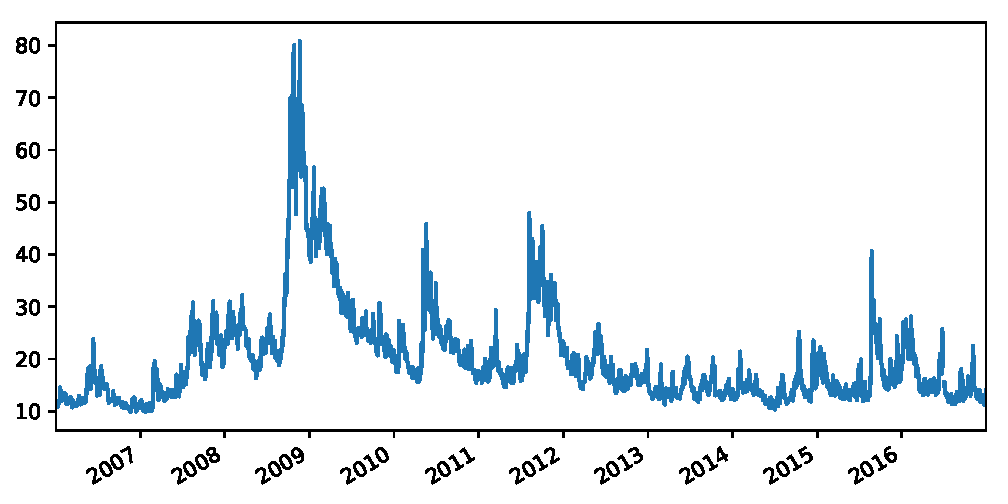
\includegraphics[width=0.8\linewidth]{vix}
	\caption[VIX from year 2006 to 2016]{Adjusted closing value of the VIX from year 2006 to 2016. Note the large spike at the end of 2008 when the global financial crisis was in full swing.}
	\label{fig:vix}
\end{figure}


\paragraph{Futures contracts} are a standard exchange-traded contract which guarantee the delivery of some underlying\footnote{%
	Because there is some underlying asset, futures belong to the family of derivative products.} 
commodity, interest rate or equity at some specified future date (expiry).\cite{wilmottwiki-futures}
They often just get called ``futures''. Because of their standardization and the resulting ease of trading, large markets formed around them. Specifically VIX futures allow for trading volatility expectations of some future date. More information about the structure of VIX futures will be presented in section~\ref{sec:aao-input-data}. One can invest in futures by placing \emph{long} or \emph{short positions}. 

By holding a long position its holder is obliged to buy the underlying assert at expiry and will hence profit from price increases. In contrast, short positions are more abstract. Their immediate meaning comes from the obligation to deliver the underlying asset at expiry. But even with no such assets at hand one can hold short positions and profit from declining prices because of the margin when purchasing its asset later. They often get abbreviated simply as ``long'' and ``short''. Intuitively it is like betting, where one can bet on rising (long) or falling (short) prices. But making such simple bets contains much risk and there are further strategies for placing these positions in a safer way.

\paragraph{Butterfly spreads} are such a strategy which will be used during this work. The general idea is simple: By mixing long and short positions on different conditions the risk of loss -- but also the profit -- gets limited. The specific usage of butterfly spreads on VIX futures gets explained in section~\ref{sec:problem-description}.

\section{Deep Learning}
\label{sec:deep-learning}

Even though the term ``deep learning'' is quite young the general architecture of its models existed for many decades. One of the first implementations might be the \emph{perceptron} by Rosenblatt in 1958. Because of its inspiration by the human brain and its connections to neuroscience the name \emph{artificial neural networks} (ANN) is most prevalent for this model family.

An especially interesting characteristic is stated in the \emph{universal approximation theorem}.\cite{Hornik-1989} It says that given enough hidden units such a network can approximate any function from one finite-dimensional space to another. But despite this theoretical representational power it is not guaranteed that one can successfully train such a network to learn the desired mapping. Because of this ANNs largely got ignored until some advantages in theory, computational power as well as larger databases allowed for breakthroughs in fields like computer vision, speech synthesis and natural language processing. With these, new interest in this model family was kindled.\cite[p.\,12ff.]{Goodfellow-et-al-2016}

\begin{figure}
	\centering
	\includegraphics[width=0.7\linewidth]{images/MultiLayerNeuralNetworkBigger_english}
	\caption[Diagram of a multi-layer feedforward artificial neural network]{%
		Diagram of a simple feedforward artificial neural network with three input nodes, one hidden layer (also with three nodes) and two output nodes. Each arrow represents a trainable weight.{\cite{wikimedia-fnn}}
	}
	\label{fig:multilayerneuralnetwork}
\end{figure}

In this work a simple architecture called \emph{feedforward neural network} (FNN), as depicted in figure~\ref{fig:multilayerneuralnetwork}, is used. In such models information only flows forward. There can be multiple hidden layers with associated weights which introduce nonlinearities. These weights are trained interatively by a technique called backpropagation where some loss function at the output of the network gets minimized by propagating the loss backwards to its beginning. The number of hidden layers is often called the \emph{depth} of a network while the maximum number of units of one such layer is called \emph{width}.

\section{Problem description}
\label{sec:problem-description}

With this, the precise definition of this thesis' goal is:

\begin{quote}
	Using the term structure and possibly additional information of a certain date to predict the corresponding spread prices of some later term.
\end{quote}

The benefit of this prediction becomes evident when looking at figure~\ref{fig:term-structure}. Most term structures have a nearly concave or convex shape. Deviations (like some small dents in the curve) are a sign of market inefficiencies that might get corrected. By investing at the right time one can gain profits if this correction takes place. A prediction might help estimating time and position of meaningful investments as well as holding time.

\begin{figure}
	\centering
	\begin{subfigure}{0.45\linewidth}
		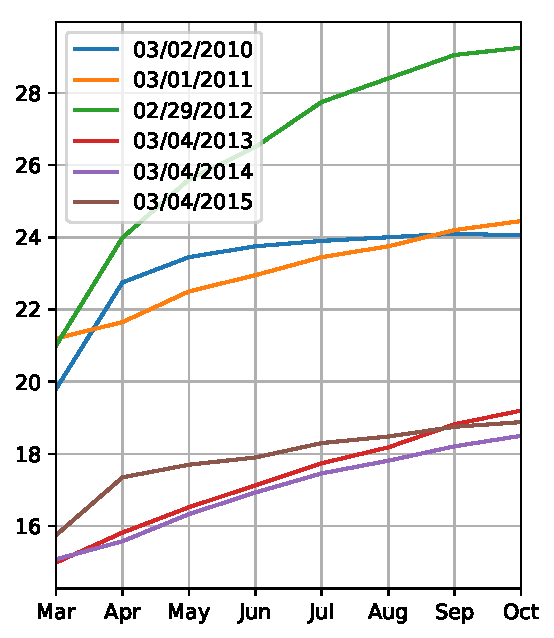
\includegraphics[width=\linewidth]{term-structure}
		\caption{}
		\label{fig:term-structure-yearly}
	\end{subfigure}
	\begin{subfigure}{0.45\linewidth}
		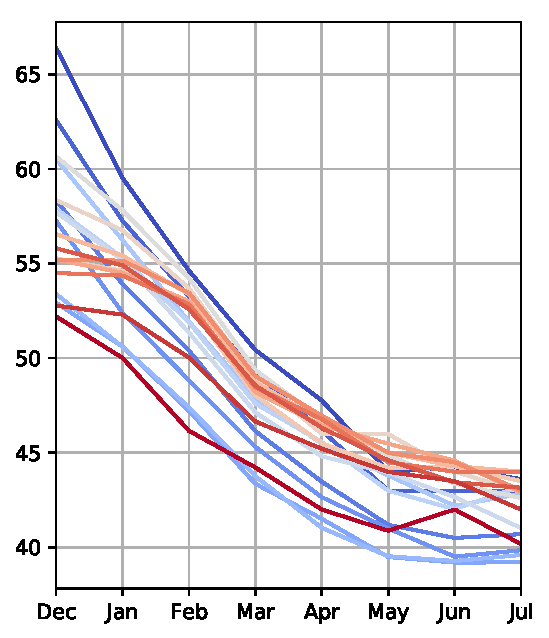
\includegraphics[width=\linewidth]{term-structure-crisis}
		\caption{}
		\label{fig:term-structure-crisis}
	\end{subfigure}\\
	\caption[Exemplary term structures of VIX futures]{%
		Exemplary term structures of VIX futures. Each line represents eight futures' prices with their month of expiration given on the x-axis. The y-axis represents their respective price. Note how in (a) each term structure is (nearly) concave. Most of the data has a similar structure. However, in time of crisis this might be different: (b) shows the term structures during November 2008, at the height of the global financial crisis. The red lines represent futures that are closer to their expiration. Their shape if often similar to convex functions. This is a form of \emph{mean reversion}{\footnotemark} where the volatility is expected to converge to some average value in the future.}
	\label{fig:term-structure}
\end{figure}
\footnotetext{A very popular and useful concept in finance as well as in daily life.}

These investments itself take place in form of butterfly spreads (intuitively described in section~\ref{sec:financial-background}). One has to distinguish between \emph{long spreads} (opening two long positions and respectively one short position at its neighboring futures) and the contrasting \emph{short spreads} (opening two short positions and respectively one long position at its neighboring futures). If there are $M$ futures' prices for a certain date and $m_i$ is the price of the $i$-th one, this results in the following definition:

\begin{subequations}
	\begin{align}
		\label{eq:long-spread}
		v^{long}_i &= 2m_i - m_{i-1} - m_{i+1} & \text{(long spread price)}
		\\
		\label{eq:short-spread}
		v^{short}_i &= -2m_i + m_{i-1} + m_{i+1} & \text{(short spread price)}
	\end{align}
\end{subequations}

One can easily see that:
\begin{equation}
	\label{eq:spread-correlation}
	v^{long}_i = -v^{short}_i 
\end{equation}
 
Moreover, there only exists a spread price for $i \in \{2,\dots,M-1\}$. In our data, most of the time a term structure of futures consists of eight prices. Therefore we have $M=8$ and six corresponding spread prices (spanning their own term structure). See figure~\ref{fig:longspread} for an example with long spreads.

\begin{figure}
	\centering
	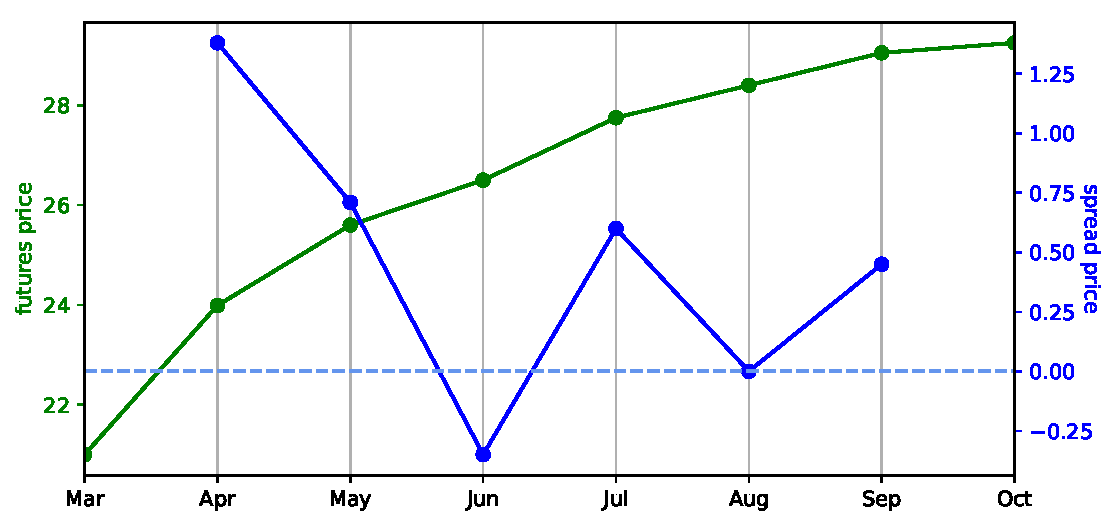
\includegraphics[width=0.8\linewidth]{images/long_spread}
	\caption[Term structure and corresponding spread prices from Feb 29, 2012]{%
		Term structure (green) and its corresponding long spread prices (blue) also forming their own term structure for February 29th, 2012.}
	\label{fig:longspread}
\end{figure}

But why use these butterfly spreads instead of investing in the futures directly? Recalling the goal of this work, it is about exploiting the term structure. Therefore the absolute value of the futures' prices is not of primary interest but the derived curvature. Butterfly spreads are a well-tried method allowing such an approach.

\newpage

When using machine learning, one has to do the following tasks: \cite{automl-2017}

\begin{enumerate}
	\item Preprocess the data
	\item Select appropriate features
	\item Select an appropriate model family
	\item Optimize model hyperparameters
	\item Postprocess machine learning models
	\item Critically analyze the results obtained
\end{enumerate}

While the title of this work already implies a model family from the subfield of deep learning -- specifically feedforward neural networks (FNNs) as mentioned in section~\ref{sec:deep-learning} -- the remaining points are determined in the course of the next chapters.

Of particular importance is the structure of the data (1. and 2.) because the remaining tasks have to be adjusted accordingly. There are two output representations this work will explore in detail: Predicting all spread prices at once (chapter~\ref{ch:all-at-once}) and predicting only a single spread price (chapter~\ref{ch:one-at-once}). The specific network structure and the corresponding hyperparameters are investigated in the respective chapters.